\documentclass{article}

\usepackage{graphicx}
\usepackage{hyperref}
\usepackage{bm}
\usepackage{float}
\restylefloat{table}

\usepackage{listings}
\usepackage{color}
\usepackage{amsmath}

\usepackage[margin=1.25in]{geometry}

\definecolor{dkgreen}{rgb}{0,0.6,0}
\definecolor{gray}{rgb}{0.5,0.5,0.5}
\definecolor{mauve}{rgb}{0.86,0.27,0.22}

\lstset{frame=tb,
  language=python,
  aboveskip=3mm,
  belowskip=3mm,
  showstringspaces=false,
  columns=flexible,
  basicstyle={\small\ttfamily},
  numbers=none,
  numberstyle=\tiny\color{gray},
  keywordstyle=\color{blue},
  commentstyle=\color{dkgreen},
  stringstyle=\color{mauve},
  breaklines=true,
  breakatwhitespace=true,
  tabsize=3
}

%----------------------------------------------------------------------------------------
%	ASSIGNMENT INFORMATION
%----------------------------------------------------------------------------------------

\title{CS5200: Homework \#4} % Title of the assignment

\author{Matthew Whitesides\\ \texttt{mbwxd4@mst.edu}} % Author name and email address

\date{\today} % University, school and/or department name(s) and a date

%----------------------------------------------------------------------------------------

\begin{document}

  \maketitle % Print the title
 
  \begin{enumerate}
    \item \textbf{10.1 Comparisons Among Lists.} \\

    \bgroup
      \def\arraystretch{1.5}
      \begin{table}[H]
        \resizebox{\textwidth}{!} {
          \begin{tabular}{lllll}
          \hline
          & \textbf{\begin{tabular}[c]{@{}l@{}}unsorted, \\ singly linked\end{tabular}} & \textbf{\begin{tabular}[c]{@{}l@{}}sorted, \\ singly linked\end{tabular}} & \textbf{\begin{tabular}[c]{@{}l@{}}unsorted, \\ doubly linked\end{tabular}} & \textbf{\begin{tabular}[c]{@{}l@{}}sorted, \\ doubly linked\end{tabular}} \\ \hline
          \textbf{SEARCH(L, k)}      & O(N) & O(N) & O(N) & O(N) \\ \hline
          \textbf{INSERT(L, x)}      & O(1) & O(N) & O(N) & O(N) \\ \hline
          \textbf{DELETE(L, x)}      & O(N) & O(N) & O(1) & O(1) \\ \hline
          \textbf{SUCCESSOR(L, x)}   & O(N) & O(1) & O(N) & O(1) \\ \hline
          \textbf{PREDECESSOR(L, x)} & O(N) & O(N) & O(N) & O(1) \\ \hline
          \textbf{MINIMUM(L)}        & O(N) & O(1) & O(N) & O(1) \\ \hline
          \textbf{MAXIMUM(L)}        & O(N) & O(N) & O(N) & O(N) \\ \hline
          \end{tabular}
        }
      \end{table}
    \egroup
    
    Note that for the two singly lists for delete we'd need an algorithm that saves the previous pointer and dosn't have to loop back around to find the previous. 
    Also I'm assuming we don't start off with having a tail pointer for any of the lists. (If we did have a tail for the lists the MAXIMUM for the two sorted would be O(1)).

    \item \textbf{11.2-2 Collision Chaining} \\
    
    $h(k) = k\;mod\;9$ \\
    $keys = 5, 28, 19, 15, 20, 33, 12, 17, 10$ \\

    \begin{table}[H]
      \begin{tabular}{l|l|llllll}
      \cline{2-2}
      0 & / & & & & & &  \\ \cline{2-8} 
      1 & $\rightarrow$ & \multicolumn{1}{l|}{28} & \multicolumn{1}{l|}{$\rightarrow$} & \multicolumn{1}{l|}{19} & \multicolumn{1}{l|}{$\rightarrow$} & \multicolumn{1}{l|}{10} & \multicolumn{1}{l|}{/} \\ \cline{2-8} 
      2 & $\rightarrow$ & \multicolumn{1}{l|}{20} & \multicolumn{1}{l|}{/}& & & &  \\ \cline{2-4}
      3 & $\rightarrow$ & \multicolumn{1}{l|}{12} & \multicolumn{1}{l|}{/}& & & &  \\ \cline{2-4}
      4 & / & & & & & &  \\ \cline{2-4}
      5 & $\rightarrow$ & \multicolumn{1}{l|}{5}  & \multicolumn{1}{l|}{/}& & & &  \\ \cline{2-6}
      6 & $\rightarrow$ & \multicolumn{1}{l|}{15} & \multicolumn{1}{l|}{$\rightarrow$} & \multicolumn{1}{l|}{33} & \multicolumn{1}{l|}{/}& &  \\ \cline{2-6}
      7 & / & & & & & &  \\ \cline{2-4}
      8 & $\rightarrow$ & \multicolumn{1}{l|}{17} & \multicolumn{1}{l|}{/}& & & &  \\ \cline{2-4}
      \end{tabular}
      \end{table}
    
    \item \textbf{11.4-1 Hash Table.}
    
    Keys = 10,22,31,4,15,28,17,88,59. \\
    Aux Hash Function: $h'(k) = k$ \\
    Linear Probing: $h(k,i) = (h'(k) + i)\;\%\;m = (k + i)\;\%\;11$. \\
    Quadratic Probing: $h(k,i) = (h'(k) + c_1i + c_2i^2)\;\%\;m = (k + 1i + 3i^2)\;\%\;11$. \\
    Double Hashing: $h(k,i) = h_1(k) + ih_2(k)\;\%\;m = k + i(1 + (k\;\%\;(m - 1)))\;\%\;m$. \\
    
    \begin{table}[H]
      \begin{tabular}{|l|l|l|l|}
      \hline
      \textbf{i}  & \textbf{Linear Probing} & \textbf{Quadratic Probing} & \textbf{Double Hashing} \\ \hline
      \textbf{0}  & 22                      & 22                         & 22                      \\ \hline
      \textbf{1}  & 88                      & /                          & /                       \\ \hline
      \textbf{2}  & /                       & 88                         & 59                      \\ \hline
      \textbf{3}  & /                       & 17                         & 17                      \\ \hline
      \textbf{4}  & 4                       & 4                          & 4                       \\ \hline
      \textbf{5}  & 15                      & /                          & 15                      \\ \hline
      \textbf{6}  & 28                      & 28                         & 28                      \\ \hline
      \textbf{7}  & 17                      & 59                         & 88                      \\ \hline
      \textbf{8}  & 59                      & 15                         & /                       \\ \hline
      \textbf{9}  & 31                      & 31                         & 31                      \\ \hline
      \textbf{10} & 10                      & 10                         & 10                      \\ \hline
      \end{tabular}
    \end{table}

    \item \textbf{12.1-1 Binary Search Trees.}
    
    Set = {1, 4, 5, 10, 16, 17, 21}

    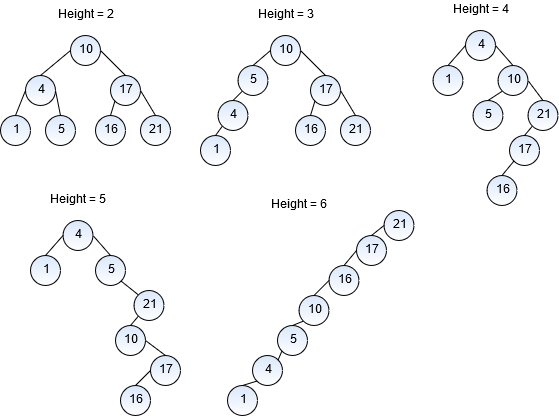
\includegraphics[width=\linewidth]{BTree.png}

    \item \textbf{12.1-2 BST v Min Heap.} 
    
    A min-heap essentially just forces the parent element above the n'th element to be smaller then it but not that left sub-trees are smaller than right subtrees. Where as a BST ensures that the n'th node has a sorted left (less than or equal) or right (greater) children. 
    Also for a BST the root does not have to be the smallest element but does for a min-heap tree. Therefore you cannot print out the sorted order of the a min-heap in O(n) time as you'd first have to sort the tree using somthing like heap sort which takes greater than n time and then print it in n time.

    \item \textbf{12.2-1 BST Search}
    
    \textbf{Option C} would be incorrect because if you follow its search to find 363 we'd go like:
    \begin{itemize}
      \item 363 $\leq$ 925 $\rightarrow$ Left
      \item 363 $\geq$ 202 $\rightarrow$ Right
      \item 363 $\leq$ 911 $\rightarrow$ Left
      \item 363 $\geq$ 240 $\rightarrow$ Right
      \item 363 $\leq$ 912 $\rightarrow$ Left* Here's the issue if you think about inserting 912 into a BST it would have been inserted to the right of 911 and not have become a child of 240. 
    \end{itemize}

    \item \textbf{Euler's Formula.} \\
    
    Let V, E, F, be the number of Verticies, Faces, and Edges. \\
    We can also say that $S + P + H = B$.
    Lets establish a couple things: 
    \begin{itemize}
        \item Euler's formula: $V - E + F = 2$.
        \item Square (S): $V = 4, E = 4$.
        \item Pentagon (P): $V = 5, E = 5$.
        \item Hexagon (H): $V = 6, E = 6$.
    \end{itemize}

    Therefore we can say that the faces F are made up of S, P, and H's and that Euler's formual can be modified as so:

    \[V - E + F = 2\]
    \[= V - E + (S + P + H) = 2\]

    Also we can say adding edges of each face of each shape in the solid, and that each edge has a shared edge with another face so if we double the edge count that'll equal the edges for each face:

    \[4S + 5P + 6H = 2E\]
    \[= 4S + 5P + 6H - 2E = 0\]
    
    And since we are saying that each vertex has three edges comming of it that:

    \[3V = 2E\]

    Now we can say that:

    \[3V - 2E = 0\]

    Subtract V from both sides:

    \[2V - 2E = -V\]

    Now using our above edge formula ($S + P + H + V - E = 2$) we can multiply it by 2 to more easily substitue in our $2V - 2E = -V$:

    \[2S + 2P + 2H + (2V - 2E) = 4\]
    \[2S + 2P + 2H + (-V) = 4\]

    Now since know we're looking for 12 we can multiply it by 3:

    \[6S + 6P + 6H - 3V = 12\]

    Also note from eariler that $4S + 5P + 6H - 2E = 0$ and that $2E = 3V$ therefore we can simply subtract this with no downside the two giving us:

    \[6S + 6P + 6H - 3V - (4S + 5P + 6H - (3V)) = 12\]

    \[= 2S + P = 12\]

    Therefore we have proven using algebra and Euler's formula that given a solid of Squares, Pentagons, and Hexagons we can say it fits the formula of $2S + P = 12$.

    \item \textbf{Program.}

  \end{enumerate}

\end{document}
